\documentclass[12pt,crop,tikz]{standalone}

\providecommand{\rootdir}{..}
\usetikzlibrary{backgrounds}
\usetikzlibrary{positioning}
\usetikzlibrary{calc}
\usetikzlibrary{decorations.pathreplacing}

\tikzstyle{arrow} = [thick,->,>=stealth]

\def\titlepad{0.1}
\def\boxspacing{40mm}

\def\layer{0.3}

\def\inner{0.3}
\def\innerspace{0.2}

\def\layerwidth{5.5cm}
\def\halflayerwidth{2.6cm}
\def\layerheight{0.8cm}
\def\innerwidth{4.4cm}
\def\halfinnerwidth{2.1cm}

% The Tableau20 colours
\definecolor{TabLightOrange}{RGB}{255,187,120}
\definecolor{TabOrange}{RGB}{255,127,14}
\definecolor{TabLightBlue}{RGB}{174,199,232}
\definecolor{TabBlue}{RGB}{31,119,180}
\definecolor{TabGreen}{RGB}{44,160,44}
\definecolor{TabLightGreen}{RGB}{152,223,138}
\definecolor{TabSalmon}{RGB}{255,152,150}
\definecolor{TabRed}{RGB}{214,39,40}
\definecolor{TabPurple}{RGB}{148,103,189}
\definecolor{TabLightPurple}{RGB}{197,176,213}
\definecolor{TabLightPink}{RGB}{247,182,210}
\definecolor{TabPink}{RGB}{227,119,194}
\definecolor{TabLightBrown}{RGB}{196,156,148}
\definecolor{TabBrown}{RGB}{140,86,75}
\definecolor{TabGray}{RGB}{127,127,127}
\definecolor{TabOlive}{RGB}{188,189,34}
\definecolor{TabLightOlive}{RGB}{219,219,141}
\definecolor{TabLightGray}{RGB}{199,199,199}
\definecolor{TabLightCyan}{RGB}{158,218,229}
\definecolor{TabCyan}{RGB}{23,190,207}

\begin{document}
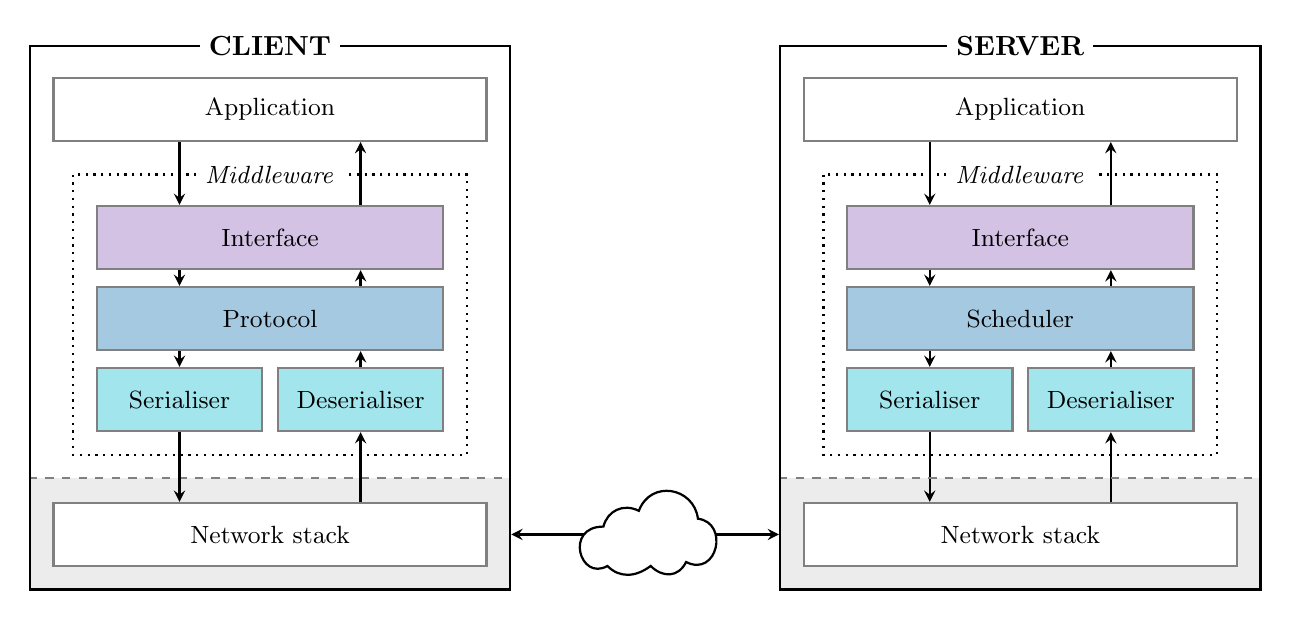
\begin{tikzpicture}
  [ every node/.style={font=\small}
  , layer/.style=    {rectangle, draw=black!50, thick, minimum width=\layerwidth    , minimum height=\layerheight}
  , halflayer/.style={rectangle, draw=black!50, thick, minimum width=\halflayerwidth, minimum height=\layerheight}
  , inner/.style=    {rectangle, draw=black!50, thick, minimum width=\innerwidth    , minimum height=\layerheight}
  , halfinner/.style={rectangle, draw=black!50, thick, minimum width=\halfinnerwidth, minimum height=\layerheight}
  , red/.style={fill=TabPurple!40}
  , orange/.style={fill=TabBlue!40}
  , yellow/.style={fill=TabCyan!40}
  , green/.style={fill=TabLightGreen!60}
  , node distance = 0cm
	, arrow={->,>=stealth}
  ]

  %-----------------------------------------------------------------------------
  %   Conventional client-side stack
  %-----------------------------------------------------------------------------

  \begin{scope}[local bounding box=std-client]
    \node[layer] (std-client-app) {Application};
    
    % hack to get the spacing right
    \coordinate (std-spaced_app1) at ($ (std-client-app.south)+(0,-\inner) $); 

    \begin{scope}[local bounding box=std-rpc-client]
      \node[inner, red, below = \layer of std-spaced_app1, yshift=-0.2cm] (std-rpc1) {Interface};
      \node[inner, orange, below = 2mm of std-rpc1] (std-rpc2) {Protocol};

      \node[halfinner, yellow, below = 2mm of std-rpc2, xshift=-1.15cm] (std-rpc3a) {Serialiser};
      \node[halfinner, yellow, below = 2mm of std-rpc2, xshift= 1.15cm] (std-rpc3b) {Deserialiser};
    \end{scope}

    \coordinate (std-rpc1-nw) at ($ (std-rpc-client.north west) + (-0.3, 0.3 + \titlepad) $);
    \coordinate (std-rpc1-ne) at ($ (std-rpc-client.north east) + ( 0.3, 0.3 + \titlepad) $);
    \coordinate (std-rpc1-sw) at ($ (std-rpc-client.south west) + (-0.3,-0.3) $);
    \coordinate (std-rpc1-se) at ($ (std-rpc-client.south east) + ( 0.3,-0.3) $);

    \draw[draw,thick,dotted] (std-rpc1-nw) rectangle (std-rpc1-se);
    \node[rectangle,fill=white] at ($(std-rpc1-nw)!0.5!(std-rpc1-ne)$) (std-rpc1_label) {\textit{Middleware}};
    
    \coordinate (std-rpc-bottom) at ($(std-rpc-client.south west)!0.5!(std-rpc-client.south east) + (0, -0.3)$);
    \node[layer, fill=white, below = 2*\layer of std-rpc-bottom] (std-Db) {Network stack};
    
    % Lines down the left
    \coordinate (std-lline) at (std-rpc3a);
    \draw[->] (std-lline |- 0, 0 |- std-client-app.south) -- (std-lline |- 0, 0 |- std-rpc1.north);
    \draw[->] (std-lline |- 0, 0 |- std-rpc1.south) -- (std-lline |- 0, 0 |- std-rpc2.north);
    \draw[->] (std-lline |- 0, 0 |- std-rpc2.south) -- (std-lline |- 0, 0 |- std-rpc3a.north);

    % Lines down the right
    \coordinate (std-rline) at (std-rpc3b);
    \draw[->] (std-rline |- 0, 0 |- std-rpc1.north) -- (std-rline |- 0, 0 |- std-client-app.south);
    \draw[->] (std-rline |- 0, 0 |- std-rpc2.north) -- (std-rline |- 0, 0 |- std-rpc1.south);
    \draw[->] (std-rline |- 0, 0 |- std-rpc3a.north) -- (std-rline |- 0, 0 |- std-rpc2.south);
    
  \end{scope}

  \begin{scope}[local bounding box=std-client-kernel]
    \fill[gray!15] ($ (std-Db.north west) + (-\layer,\layer) $) rectangle ($ (std-Db.south east) + (\layer, -\layer) $);
  \end{scope}
  \draw[-, gray, dashed] (std-client-kernel.north west) -- (std-client-kernel.north east);

  \node[layer, fill=white, below = 2*\layer of std-rpc-bottom] (std-Db) {Network stack};
  \draw[->] (std-lline |- 0, 0 |- std-rpc3a.south) -- (std-lline |- 0, 0 |- std-Db.north);
  \draw[<-] (std-rline |- 0, 0 |- std-rpc3b.south) -- (std-rline |- 0, 0 |- std-Db.north);
  
  \coordinate (std-client-nw) at ($ (std-client.north west) + (-\inner, \inner + \titlepad) $);
  \coordinate (std-client-ne) at ($ (std-client.north east) + ( \inner, \inner + \titlepad) $);
  \coordinate (std-client-sw) at ($ (std-client.south west) + (-\inner,-\inner) $);
  \coordinate (std-client-se) at ($ (std-client.south east) + ( \inner,-\inner) $);
    
  \draw[draw, thick] (std-client-nw) rectangle (std-client-se);
  \node[rectangle, fill=white] at ($(std-client-nw)!0.5!(std-client-ne)$) (std-client_label) {\normalsize\textbf{CLIENT}};
  
  %-----------------------------------------------------------------------------
  %   CausalRPC client-side stack
  %   -----------------------------------------------------------------------------

  \begin{scope}[local bounding box=client]
    % \coordinate[right=5cm of std-client-] (client_center)
    
    \node[layer, right = 4cm of std-client-app] (client-app) {Application};
    
    % hack to get the spacing right
    \coordinate (spaced_app1) at ($ (client-app.south)+(0,-\inner) $); 

    \begin{scope}[local bounding box=rpc-client]
      \node[inner, red, below = \layer of spaced_app1, yshift=-0.2cm] (rpc1) {Interface};
      \node[inner, orange, below = 2mm of rpc1] (rpc2) {Scheduler};

      \node[halfinner, yellow, below = 2mm of rpc2, xshift=-1.15cm] (rpc3a) {Serialiser};
      \node[halfinner, yellow, below = 2mm of rpc2, xshift= 1.15cm] (rpc3b) {Deserialiser};
    \end{scope}

    \coordinate (rpc1-nw) at ($ (rpc-client.north west) + (-0.3, 0.3 + \titlepad) $);
    \coordinate (rpc1-ne) at ($ (rpc-client.north east) + ( 0.3, 0.3 + \titlepad) $);
    \coordinate (rpc1-sw) at ($ (rpc-client.south west) + (-0.3,-0.3) $);
    \coordinate (rpc1-se) at ($ (rpc-client.south east) + ( 0.3,-0.3) $);

    \draw[draw,thick,dotted] (rpc1-nw) rectangle (rpc1-se);
    \node[rectangle,fill=white] at ($(rpc1-nw)!0.5!(rpc1-ne)$) (rpc1_label) {\textit{Middleware}};
    
    \coordinate (rpc-bottom) at ($(rpc-client.south west)!0.5!(rpc-client.south east) + (0, -0.3)$);
    \node[layer, fill=white, below = 2*\layer of rpc-bottom] (Db) {Network stack};
    
    % Lines down the left
    \coordinate (lline) at (rpc3a);
    \draw[->] (lline |- 0, 0 |- client-app.south) -- (lline |- 0, 0 |- rpc1.north);
    \draw[->] (lline |- 0, 0 |- rpc1.south) -- (lline |- 0, 0 |- rpc2.north);
    \draw[->] (lline |- 0, 0 |- rpc2.south) -- (lline |- 0, 0 |- rpc3a.north);
    \draw[->] (lline |- 0, 0 |- rpc3a.south) -- (lline |- 0, 0 |- Db.north);

    % Lines down the right
    \coordinate (rline) at (rpc3b);
    \draw[->] (rline |- 0, 0 |- rpc1.north) -- (rline |- 0, 0 |- client-app.south);
    \draw[->] (rline |- 0, 0 |- rpc2.north) -- (rline |- 0, 0 |- rpc1.south);
    \draw[->] (rline |- 0, 0 |- rpc3a.north) -- (rline |- 0, 0 |- rpc2.south);
    \draw[->] (rline |- 0, 0 |- Db.north) -- (rline |- 0, 0 |- rpc3a.south);
  \end{scope}

  \begin{scope}[on background layer, local bounding box=client-kernel]
    \fill[gray!15] ($ (Db.north west) + (-\layer,\layer) $) rectangle ($ (Db.south east) + (\layer, -\layer) $);
  \end{scope}
  
  \draw[-, gray, dashed] (client-kernel.north west) -- (client-kernel.north east);

  \coordinate (client-nw) at ($ (client.north west) + (-\inner, \inner + \titlepad) $);
  \coordinate (client-ne) at ($ (client.north east) + ( \inner, \inner + \titlepad) $);
  \coordinate (client-sw) at ($ (client.south west) + (-\inner,-\inner) $);
  \coordinate (client-se) at ($ (client.south east) + ( \inner,-\inner) $);
    
  \draw[draw, thick] (client-nw) rectangle (client-se);
  \node[rectangle, fill=white] at ($(client-nw)!0.5!(client-ne)$) (client_label) {\normalsize\textbf{SERVER}};
  

  \coordinate (net-left) at ($(Db.north west)!0.3333!(Db.north east)$);
  \coordinate (net-right) at ($(Db.north west)!0.6667!(Db.north east)$);
  % \draw[->] (net-left |- 0, 0 |- git.south) -- (net-left |- 0, 0 |- Db.north);
  % \draw[<-] (net-right |- 0, 0 |- git.south) -- (net-right |- 0, 0 |- Db.north);

  \draw[<->] ($ (std-Db.east) + (\inner,0) $) -- ($ (Db.west) + (-\inner, 0) $);
  
  \coordinate (cloud_center) at ($(std-Db.east)!0.58!(Db.west)$);
  \begin{scope}[local bounding box=cloud,shift={($(cloud_center) + (0, -0.05)$)}, rotate=0, scale=0.5]
    \draw[fill=white,thick] (-1.6,-0.7) .. controls (-2.3,-1.1)
    and (-2.7,0.3) .. (-1.7,0.3) .. controls (-1.6,0.7)
    and (-1.2,0.9) .. (-0.8,0.7) .. controls (-0.5,1.5)
    and (0.6,1.3) .. (0.7,0.5) .. controls (1.5,0.4)
    and (1.2,-1) .. (0.4,-0.6) .. controls (0.2,-1)
    and (-0.2,-1) .. (-0.5,-0.7) .. controls (-0.9,-1)
    and (-1.3,-1) .. cycle;
  \end{scope}


\end{tikzpicture}
\end{document}